\documentclass[11pt]{article}
\usepackage{csc766}

%%%%%%%%%%%%%%%%%%%% name/id
\rfoot{\small Brian Park | 200190057}


%%%%%%%%%%%%%%%%%%%% Course/HW info
\newcommand*{\instr}{Xipeng Shen}
\newcommand*{\term}{Spring 2023}
\newcommand*{\coursenum}{CSC 766}
\newcommand*{\coursename}{Code Optimization for Scalar and Parallel Programs}
\newcommand*{\hwnum}{1}

\rhead{\LARGE   \fontfamily{lmdh}\selectfont	HW \hwnum}

\lfoot{\small \coursenum, \term, HW \hwnum}

%%%%%%%%%%%%%%%%%%%%%%%%%%%%%% Document Start %%%%%%%%%%%%%%%%%
\begin{document}

%%%%%%%%%%%%%%%%%%%%%%%%%%%%%%%%%%%%%%%%%%%%%%%%%%%%%%%%%%%%%%%%%%%%%%%%%%%%%%%%%%%%%%%%
% Question 1
%%%%%%%%%%%%%%%%%%%%%%%%%%%%%%%%%%%%%%%%%%%%%%%%%%%%%%%%%%%%%%%%%%%%%%%%%%%%%%%%%%%%%%%%
\section{}

Answer questions based on the CFG below:
\begin{figure}[H]
	\centerline{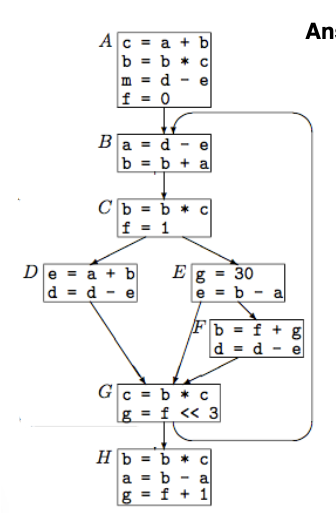
\includegraphics[width=2in]{figures/hw1_cfg1.png}}
\end{figure}

\begin{enumerate}
	\item Find the extended basic blocks.
	      \begin{Answer}
		      The EBBs are:
		      \{A\}, \{B\}, \{C\}, \{D\}, \{E\}, \{F\}, \{G\}, \{H\}, \{BC\}, \{CD\}, \{CE\}, \{EF\}, \{BCD\}, \{BCE\}, \{CEF\}, \{CDE\}, \{BCDE\}, \{BCEF\}, \{CDEF\}, \{BCDEF\}, \{GH\}.

		      But more concisely (to help with value numbering), they can be defined as: \{A\}, \{BCDEF\}, \{GH\}.
	      \end{Answer}
	\item Find the dominator set for each basic block.
	      \begin{Answer}
		      \begin{center}
			      \begin{tabular}{ |c|c|c| }
				      \hline
				      Block & Dom           & IDom \\ [0.5ex] % inserts table
				      \hline
				      A     & A             & -    \\
				      B     & A, B          & A    \\
				      C     & A, B, C       & B    \\
				      D     & A, B, C, D    & C    \\
				      E     & A, B, C, E    & C    \\
				      F     & A, B, C, E, F & E    \\
				      G     & A, B, C, G    & C    \\
				      H     & A, B, C, G, H & G    \\
				      \hline
			      \end{tabular}
		      \end{center}
	      \end{Answer}
	\item Build the dominance tree.
	      \begin{Answer}
		      \begin{verbatim}
  A
  |
  B
  |
  C
/ | \
D E G
  | |
  F H
\end{verbatim}
	      \end{Answer}
	\item Apply super local numbering to the CFG.
	      \begin{Answer}
		      Super local value numbering is as follows:
		      \begin{enumerate}[i]
			      \item Build SSA form
			      \item Find EBBs
			      \item Apply value numbering to each path in each EBB using scoped hash tables
		      \end{enumerate}

		      First, we can rewrite the each basic block in SSA form as follows: \\ \\
		      \textbf{Block A}: \\
		      $c_0 = a_0 + b_1$ \\
		      $b_1 = b_0 * c_0$ \\
		      $m_0 = d_0 - e_0$ \\
		      $f_0 = 0$ \\
		      \textbf{Block B}: \\
		      $b_2 = \phi(b_1, b_6)$ \\
		      $c_1 = \phi(c_0, c_2)$ \\
		      $d_1 = \phi(d_0, d_4)$ \\
		      $e_1 = \phi(e_0, e_4)$ \\
		      $f_1 = \phi(f_0, f_2)$ \\
		      $g_1 = \phi(g_0, g_4)$ \\
		      $a_1 = d_1 - e_1$ \\
		      $b_3 = b_2 + a_1$ \\
		      \textbf{Block C}: \\
		      $b_4 = b_3 * c_1$ \\
		      $f_2 = 1$ \\
		      \textbf{Block D}: \\
		      $e_2 = a_1 + b_4$ \\
		      $d_2 = d_1 - e_2$ \\
		      \textbf{Block E}: \\
		      $g_2 = 30$ \\
		      $e_3 = b_4 - a_1$ \\
		      \textbf{Block F}: \\
		      $b_5 = f_2 + g_2$ \\
		      $d_3 = d_1 - e_3$ \\
		      \textbf{Block G}: \\
		      $b_6 = \phi(b_5, b_4, b_4)$ \\
		      $d_4 = \phi(d_1, d_2, d_3)$ \\
		      $e_4 = \phi(e_2, e_3, e_3)$ \\
		      $g_3 = \phi(g_1, g_2, g_2)$ \\
		      $c_2 = b_6 * c_1$ \\
		      $g_4 = f_2 << 3$ \\
		      \textbf{Block H}: \\
		      $b_7 = b_6 * c_2$ \\
		      $a_2 = b_7 - a_1$ \\
		      $g_5 = f_2 + 1$ \\


		      Second, we find EBBs, which were already derived before. But now, we only consider the paths, which are A, BCDEF, GH.

		      Lastly, we apply value numbering to each path in the EBB using scoped hash tables (Value numbers are denoted as superscripts). \\
		      \textbf{EBB Path: A} \\
		      \textbf{Block A}: \\
		      $c_0^2 = a_0^0 + b_1^1$ \\
		      $b_1^3 = b_0^1 * c_0^2$ \\
		      $m_0^6 = d_0^4 - e_0^5$ \\
		      $f_0^8 = 0^7$ \\
		      \\
		      \textit{No values redundant} \\

		      \textbf{EBB Path: BCDEF} \\
		      \textbf{Block B}: \\
		      $b_2^2 = \phi(b_1^0, b_6^1)$ \\
		      $c_1^5 = \phi(c_0^3, c_2^4)$ \\
		      $d_1^8 = \phi(d_0^6, d_4^7)$ \\
		      $e_1^{11} = \phi(e_0^9, e_4^{10})$ \\
		      $f_1^{14} = \phi(f_0^{12}, f_2^{13})$ \\
		      $g_1^{17} = \phi(g_0^{15}, g_4^{16})$ \\
		      $a_1^{18} = d_1^8 - e_1^{11}$ \\
		      $b_3^{19} = b_2^2 + a_1^{18}$ \\
		      \textbf{Block C}: \\
		      $b_4^{20} = b_3^{19} * c_1^5$ \\
		      $f_2^{22} = 1^{21}$ \\
		      \textbf{Block D}: \\
		      $e_2^{23} = a_1^{18} + b_4^{20}$ \\
		      $d_2^{24} = d_1^{8} - e_2^{23}$ \\
		      \textbf{Block E}: \\
		      $g_2^{26} = 30^{25}$ \\
		      $e_3^{27} = b_4^{20} - a_1^{18}$ \\
		      \textbf{Block F}: \\
		      $b_5^{28} = f_2^{22} + g_2^{26}$ \\
		      $d_3^{29} = d_1^{8} - e_3^{27}$ \\
		      \\
		      \textit{No values redundant} \\

		      \textbf{EBB Path: GH} \\
		      \textbf{Block G}: \\
		      $b_6^3 = \phi(b_5^0, b_4^1, b_4^2)$ \\
		      $d_4^7 = \phi(d_1^4, d_2^5, d_3^6)$ \\
		      $e_4^{11} = \phi(e_2^8, e_3^9, e_3^{10})$ \\
		      $g_3^{15} = \phi(g_1^{12}, g_2^{13}, g_2^{14})$ \\
		      $c_2^{17} = b_6^3 * c_1^{16}$ \\
		      $g_4^{20} = f_2^{18} << 3^{19}$ \\
		      \textbf{Block H}: \\
		      $b_7^{18} = b_6^3 * c_2^{17}$ \\
		      $a_2^{19} = b_7^{18} - a_1^{19}$ \\
		      $g_5^{22} = f_2^{20} + 1^{21}$ \\
		      \\
		      \textit{No values redundant} \\

		      In the end, unfortunately there are no values to be rewritten.
	      \end{Answer}
	\item Apply dominator-based value numbering to the CFG.
	      \begin{Answer}
		      Dominator-based value numbering is as follows:
		      \begin{enumerate}[i]
			      \item Build SSA form
			      \item Use table from IDom($x$) to start value numbering
			      \item Follow the order of IDOM tree
		      \end{enumerate}

		      We have already built SSA form from the previous question, so we can get straight into using the IDom table to do value numbering. Thus, the scopes to do value numbering based on their IDOM($x$) is as follows:
		      $\{A\}, \{A, B\}, \{B, C\}, \{C, D\}, \{C, E\}, \{E, F\}, \{C, G\}, \{G, H\} $
		      \\ \\
		      \textbf{Scope} $\{A\}$ \\
		      \textbf{Block A}: \\
		      $c_0^2 = a_0^0 + b_1^1$ \\
		      $b_1^3 = b_0^1 * c_0^2$ \\
		      $m_0^6 = d_0^4 - e_0^5$ \\
		      $f_0^8 = 0^7$ \\
		      \\
		      \textit{No values redundant} \\
		      \\
		      \textbf{Scope} $\{A, B\}$ \\
		      \textbf{Block A}: \\
		      $c_0^2 = a_0^0 + b_1^1$ \\
		      $b_1^3 = b_0^1 * c_0^2$ \\
		      $m_0^6 = d_0^4 - e_0^5$ \\
		      $f_0^8 = 0^7$ \\

		      \textbf{Block B}: \\
		      $b_2^2 = \phi(b_1^0, b_6^1)$ \\
		      $c_1^5 = \phi(c_0^3, c_2^4)$ \\
		      $d_1^8 = \phi(d_0^6, d_4^7)$ \\
		      $e_1^{11} = \phi(e_0^9, e_4^{10})$ \\
		      $f_1^{14} = \phi(f_0^{12}, f_2^{13})$ \\
		      $g_1^{17} = \phi(g_0^{15}, g_4^{16})$ \\
		      $a_1^{18} = d_1^8 - e_1^{11}$ \\
		      $b_3^{19} = b_2^2 + a_1^{18}$ \\
		      \\
		      \textit{No values redundant} \\
		      \\

		      Scope $\{B, C\}$ \\
		      \textbf{Block B}: \\
		      $b_2^2 = \phi(b_1^0, b_6^1)$ \\
		      $c_1^5 = \phi(c_0^3, c_2^4)$ \\
		      $d_1^8 = \phi(d_0^6, d_4^7)$ \\
		      $e_1^{11} = \phi(e_0^9, e_4^{10})$ \\
		      $f_1^{14} = \phi(f_0^{12}, f_2^{13})$ \\
		      $g_1^{17} = \phi(g_0^{15}, g_4^{16})$ \\
		      $a_1^{18} = d_1^8 - e_1^{11}$ \\
		      $b_3^{19} = b_2^2 + a_1^{18}$ \\
		      \textbf{Block C}: \\
		      $b_4^{20} = b_3^{19} * c_1^5$ \\
		      $f_2^{22} = 1^{21}$ \\
		      \\
		      \textit{No values redundant} \\
		      \\

		      Scope $\{C, D\}$ \\
		      \textbf{Block C}: \\
		      $b_4^2 = b_3^0 * c_1^1$ \\
		      $f_2^4 = 1^3$ \\
		      \textbf{Block D}: \\
		      $e_2^6 = a_1^5 + b_4^2$ \\
		      $d_2^8 = d_1^7 - e_2^6$ \\
		      \\
		      \textit{No values redundant} \\
		      \\

		      Scope $\{C, E\}$ \\
		      \textbf{Block C}: \\
		      $b_4^2 = b_3^0 * c_1^1$ \\
		      $f_2^4 = 1^3$ \\
		      \textbf{Block E}: \\
		      $g_2^6 = 30^5$ \\
		      $e_3^8 = b_4^2 - a_1^7$ \\
		      \\
		      \textit{No values redundant} \\
		      \\

		      Scope $\{E, F\}$ \\
		      \textbf{Block E}: \\
		      $g_2^1 = 30^0$ \\
		      $e_3^4 = b_4^3 - a_1^2$ \\
		      \textbf{Block F}: \\
		      $b_5^6 = f_2^5 + g_2^1$ \\
		      $d_3^8 = d_1^7 - e_3^4$ \\
		      \\
		      \textit{No values redundant} \\
		      \\

		      Scope $\{C, G\}$ \\
		      \textbf{Block C}: \\
		      $b_4^2 = b_3^0 * c_1^1$ \\
		      $f_2^4 = 1^3$ \\
		      \textbf{Block D}: \\
		      $e_2^6 = a_1^5 + b_4^2$ \\
		      $d_2^8 = d_1^7 - e_2^6$ \\
		      \textbf{Block E}: \\
		      $g_2^{10} = 30^9$ \\
		      $e_3^{11} = b_4^2 - a_1^5$ \\
		      \textbf{Block F}: \\
		      $b_5^{12} = f_2^4 + g_2^{10}$ \\
		      $d_3^{13} = d_1^7 - e_3^{11}$ \\
		      \textbf{Block G}: \\
		      $b_6^{14} = \phi(b_5^{12}, b_4^{2}, b_4{2})$ \\
		      $d_4^{15} = \phi(d_1^7, d_2^8, d_3^{13})$ \\
		      $e_4^{16} = \phi(e_2^6, e_3^{13}, e_3^{13})$ \\
		      $g_3^{17} = \phi(g_1^{18}, g_2^{10}, g_2^{10})$ \\
		      $c_2^{19} = b_6^{14} * c_1^1$ \\
		      $g_4^{21} = f_2^4 << 3^{20}$ \\
		      \\
		      \textit{No values redundant} \\
		      \\

		      Scope $\{G, H\}$ \\
		      \textbf{Block G}: \\
		      $b_6^3 = \phi(b_5^0, b_4^1, b_4^2)$ \\
		      $d_4^7 = \phi(d_1^4, d_2^5, d_3^6)$ \\
		      $e_4^{11} = \phi(e_2^8, e_3^9, e_3^{10})$ \\
		      $g_3^{15} = \phi(g_1^{12}, g_2^{13}, g_2^{14})$ \\
		      $c_2^{17} = b_6^3 * c_1^{16}$ \\
		      $g_4^{20} = f_2^{18} << 3^{19}$ \\
		      \textbf{Block H}: \\
		      $b_7^{18} = b_6^3 * c_2^{17}$ \\
		      $a_2^{19} = b_7^{18} - a_1^{19}$ \\
		      $g_5^{22} = f_2^{20} + 1^{21}$ \\
		      \\
		      \textit{No values redundant} \\

		      Again, unfortunately no values were rewritten. There were close enough values to be rewritten, but because of the renaming via SSA, it was not possible.
	      \end{Answer}
\end{enumerate}

\newpage
\section{}
\begin{figure}[H]
	\centerline{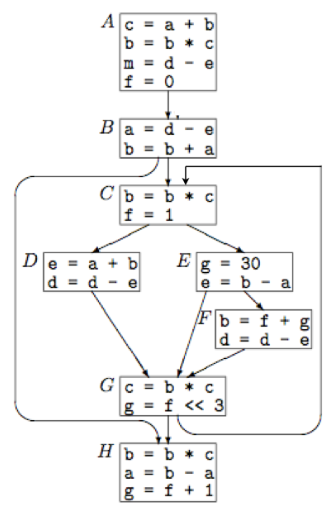
\includegraphics[width=2in]{figures/hw1_cfg2.png}}
\end{figure}
In our lecture, we learned how to compute $LIVEOUT$ set for every basic block. In this exercise, you are asked to come up a way to compute $LIVEIN$, which is the set of variables that are live at the entry point of a basic block. Specifically, you are asked to:

\begin{enumerate}
	\item Clearly describe your algorithm
	      \begin{Answer}
		      First we'll define some notation:
		      \begin{itemize}
			      \item $LIVEIN(n)$ contains the name of every variable that is live on entry to $n$
			      \item $UEVAR(n)$ contains the upward-exposed variables in $n$, i.e. those that are used in $n$ before any redefinition in $n$
			      \item $VARKILL(n)$ contains all the variables that are defined in $n$
			      \item $n_f$ is the exit node of the CFG
		      \end{itemize}
		      $$LIVEIN(n_f) = UEVar(n_f)$$
		      $$LIVEIN(n) = (\bigcup_{m \in succ(n)} LIVEIN(m) \cap \overline{VARKILL(n)}) \cup UEVar(n)$$
	      \end{Answer}
	\item Indicate the order of traversing a CFG for your algorithm to work efficiently
	      \begin{Answer}
		      The order of traversing of CFG is backwards or in postorder. It is optimal to visit children before parents.
	      \end{Answer}
	\item Solve LIVEIN for the following CFG. You need to give the local sets values for the basic
	      blocks, and the final results of the LIVEIN sets of the CFG.
	      \begin{Answer}
		      Here are some local set values: \\
		      $UEVar(A) = \{a, b, c, d, e\}$ \\
		      $UEVar(B) = \{a, b, d, e\}$ \\
		      $UEVar(C) = \{b, c\}$ \\
		      $UEVar(D) = \{a, b, d, e\}$ \\
		      $UEVar(E) = \{a, b\}$ \\
		      $UEVar(F) = \{d, e, f, g\}$ \\
		      $UEVar(G) = \{b, c, f\}$ \\
		      $UEVar(H) = \{a, b, c, f\}$ \\

		      $VarKill(A) = \{b, c, f, m\}$ \\
		      $VarKill(B) = \{a, b\}$ \\
		      $VarKill(C) = \{b, f\}$ \\
		      $VarKill(D) = \{d, e\}$ \\
		      $VarKill(E) = \{e, g\}$ \\
		      $VarKill(F) = \{b, d\}$ \\
		      $VarKill(G) = \{c, g\}$ \\
		      $VarKill(H) = \{a, b, g\}$ \\

		      Thus, using the algorithm above, we can define the $LIVEIN$ sets as (it took three iterations for the sets to finally converge): \\
		      $LiveIn(A) = \{a, b, c, d, e, f, g\}$ \\
		      $LiveIn(B) = \{a, b, c, d, e, f, g\}$ \\
		      $LiveIn(C) = \{a, b, c, d, e, f, g\}$ \\
		      $LiveIn(D) = \{a, b, c, d, e, f, g\}$ \\
		      $LiveIn(E) = \{a, b, c, d, f\}$ \\
		      $LiveIn(F) = \{a, b, c, d, e, f, g\}$ \\
		      $LiveIn(G) = \{a, b, c, d, e, f\}$ \\
		      $LiveIn(H) = \{a, b, c, f\}$ \\
	      \end{Answer}
\end{enumerate}

\end{document}